% Options for packages loaded elsewhere
\PassOptionsToPackage{unicode}{hyperref}
\PassOptionsToPackage{hyphens}{url}
\PassOptionsToPackage{dvipsnames,svgnames,x11names}{xcolor}
%
\documentclass[
  11pt,
  a4paper,
  DIV=11,
  numbers=noendperiod]{scrartcl}

\usepackage{amsmath,amssymb}
\usepackage{iftex}
\ifPDFTeX
  \usepackage[T1]{fontenc}
  \usepackage[utf8]{inputenc}
  \usepackage{textcomp} % provide euro and other symbols
\else % if luatex or xetex
  \usepackage{unicode-math}
  \defaultfontfeatures{Scale=MatchLowercase}
  \defaultfontfeatures[\rmfamily]{Ligatures=TeX,Scale=1}
\fi
\usepackage{lmodern}
\ifPDFTeX\else  
    % xetex/luatex font selection
  \setmainfont[]{Avenir Next}
\fi
% Use upquote if available, for straight quotes in verbatim environments
\IfFileExists{upquote.sty}{\usepackage{upquote}}{}
\IfFileExists{microtype.sty}{% use microtype if available
  \usepackage[]{microtype}
  \UseMicrotypeSet[protrusion]{basicmath} % disable protrusion for tt fonts
}{}
\makeatletter
\@ifundefined{KOMAClassName}{% if non-KOMA class
  \IfFileExists{parskip.sty}{%
    \usepackage{parskip}
  }{% else
    \setlength{\parindent}{0pt}
    \setlength{\parskip}{6pt plus 2pt minus 1pt}}
}{% if KOMA class
  \KOMAoptions{parskip=half}}
\makeatother
\usepackage{xcolor}
\setlength{\emergencystretch}{3em} % prevent overfull lines
\setcounter{secnumdepth}{-\maxdimen} % remove section numbering
% Make \paragraph and \subparagraph free-standing
\ifx\paragraph\undefined\else
  \let\oldparagraph\paragraph
  \renewcommand{\paragraph}[1]{\oldparagraph{#1}\mbox{}}
\fi
\ifx\subparagraph\undefined\else
  \let\oldsubparagraph\subparagraph
  \renewcommand{\subparagraph}[1]{\oldsubparagraph{#1}\mbox{}}
\fi


\providecommand{\tightlist}{%
  \setlength{\itemsep}{0pt}\setlength{\parskip}{0pt}}\usepackage{longtable,booktabs,array}
\usepackage{calc} % for calculating minipage widths
% Correct order of tables after \paragraph or \subparagraph
\usepackage{etoolbox}
\makeatletter
\patchcmd\longtable{\par}{\if@noskipsec\mbox{}\fi\par}{}{}
\makeatother
% Allow footnotes in longtable head/foot
\IfFileExists{footnotehyper.sty}{\usepackage{footnotehyper}}{\usepackage{footnote}}
\makesavenoteenv{longtable}
\usepackage{graphicx}
\makeatletter
\def\maxwidth{\ifdim\Gin@nat@width>\linewidth\linewidth\else\Gin@nat@width\fi}
\def\maxheight{\ifdim\Gin@nat@height>\textheight\textheight\else\Gin@nat@height\fi}
\makeatother
% Scale images if necessary, so that they will not overflow the page
% margins by default, and it is still possible to overwrite the defaults
% using explicit options in \includegraphics[width, height, ...]{}
\setkeys{Gin}{width=\maxwidth,height=\maxheight,keepaspectratio}
% Set default figure placement to htbp
\makeatletter
\def\fps@figure{htbp}
\makeatother

\usepackage[document]{ragged2e}
\KOMAoption{captions}{tableheading}
\makeatletter
\@ifpackageloaded{caption}{}{\usepackage{caption}}
\AtBeginDocument{%
\ifdefined\contentsname
  \renewcommand*\contentsname{Table of contents}
\else
  \newcommand\contentsname{Table of contents}
\fi
\ifdefined\listfigurename
  \renewcommand*\listfigurename{List of Figures}
\else
  \newcommand\listfigurename{List of Figures}
\fi
\ifdefined\listtablename
  \renewcommand*\listtablename{List of Tables}
\else
  \newcommand\listtablename{List of Tables}
\fi
\ifdefined\figurename
  \renewcommand*\figurename{Figure}
\else
  \newcommand\figurename{Figure}
\fi
\ifdefined\tablename
  \renewcommand*\tablename{Table}
\else
  \newcommand\tablename{Table}
\fi
}
\@ifpackageloaded{float}{}{\usepackage{float}}
\floatstyle{ruled}
\@ifundefined{c@chapter}{\newfloat{codelisting}{h}{lop}}{\newfloat{codelisting}{h}{lop}[chapter]}
\floatname{codelisting}{Listing}
\newcommand*\listoflistings{\listof{codelisting}{List of Listings}}
\makeatother
\makeatletter
\makeatother
\makeatletter
\@ifpackageloaded{caption}{}{\usepackage{caption}}
\@ifpackageloaded{subcaption}{}{\usepackage{subcaption}}
\makeatother
\ifLuaTeX
  \usepackage{selnolig}  % disable illegal ligatures
\fi
\usepackage{bookmark}

\IfFileExists{xurl.sty}{\usepackage{xurl}}{} % add URL line breaks if available
\urlstyle{same} % disable monospaced font for URLs
\hypersetup{
  pdftitle={TKInter},
  colorlinks=true,
  linkcolor={blue},
  filecolor={Maroon},
  citecolor={Blue},
  urlcolor={Blue},
  pdfcreator={LaTeX via pandoc}}

\title{TKInter}
\author{}
\date{}

\begin{document}
\maketitle

\begin{itemize}
\tightlist
\item
  Es gibt APIs = Application Programming Interface
\item
  für GUIs = Graphical Use Interface
\item
  in Python gibt es tkinter (relativ einfach)
\item
  alternativ aber komplizierter sind PyGtk, PyQT, \ldots{}
\item
  unser Ziel: Visualisierung unserer geometrischen Objekte.
\end{itemize}

\subsubsection{Fenster}\label{fenster}

\begin{enumerate}
\def\labelenumi{\arabic{enumi}.}
\item
  tkinter wird importiert
\item
  mit Hife des Tk()-Konstruktors wird ein Wurzelobjekt erzeugt.
\end{enumerate}

\begin{itemize}
\tightlist
\item
  Diese Wurzelobjekt ist ein Fenster.
\item
  Zu diesem Objekt können weitere Bestandteile zugefügt werden.
\end{itemize}

\begin{enumerate}
\def\labelenumi{\arabic{enumi}.}
\setcounter{enumi}{2}
\tightlist
\item
  \texttt{lab} repräsentiert ein Label-Widget.
\end{enumerate}

\begin{itemize}
\tightlist
\item
  Das Label wird dem Wurzelelement hinzugefügt.
\item
  Widget = rechteckige Fläche auf dem Bildschirm mit einer
  Funktionalität
\item
  Label-Widget kann nur Text anzeigen.
\end{itemize}

\begin{enumerate}
\def\labelenumi{\arabic{enumi}.}
\setcounter{enumi}{3}
\tightlist
\item
  Anordnung des Widgets im Fenster
\end{enumerate}

\begin{itemize}
\tightlist
\item
  Vorgefertigte
\end{itemize}

\subsubsection{Canvas}\label{canvas}

\begin{enumerate}
\def\labelenumi{\arabic{enumi}.}
\tightlist
\item
  Canvas dem Fenster
\end{enumerate}

\begin{itemize}
\tightlist
\item
  Canvas ist ein Widget
\item
  Canvas = Leinwand
\item
  Auf Canvas können geometrische Figuren gemalt werden.
\item
  Der Konstruktor \texttt{tk.Canvas()} übernimmt als Parameter Breite
  und Höhe in Pixeln
\end{itemize}

\begin{enumerate}
\def\labelenumi{\arabic{enumi}.}
\setcounter{enumi}{1}
\tightlist
\item
  Auf dem Canvas malen
\end{enumerate}

\subsubsection{Graphikkoordinaten}\label{graphikkoordinaten}

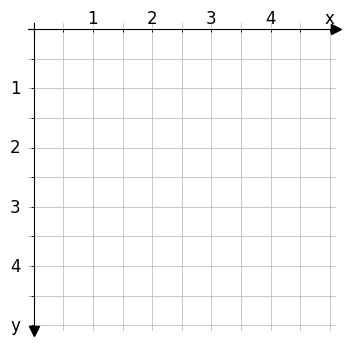
\includegraphics{/Users/martin/Workspace/Jupyter_Notebooks/Info_KS/2_Objectoriented_Programming/2-4_GUI-Programming/images/coordinates.png}

\subsubsection{Canvas Methoden}\label{canvas-methoden}

\begin{itemize}
\item
  Linie von (x1, y1) nach (x2, y2)\\
  \texttt{canvas.create\_line(x1,\ y1,\ x2,\ y2,\ **options)}
\item
  Rechteck von obere linke Ecke (x1, y1) nach untere rechte Ecke (x2,
  y2)\\
  \texttt{canvas.create\_rectangle(x1,\ y1,\ x2,\ y2,\ **options)}
\item
  Oval innerhalb des Rechtecks gebildet durch obere linke Ecke (x1, y1)
  und untere rechte Ecke (x2, y2)\\
  \texttt{canvas.create\_oval(x1,\ y1,\ x2,\ y2,\ **options)}
\end{itemize}

=\textgreater{} Alle \texttt{create}-Methoden liefern den Index des
erzeugten Objekts\\
= Eindeutige Referenz auf das Objekt. - Damit kann das Objekt noch
nachträglich geändert werden.



\end{document}
